\documentclass[twoside]{article}

% Packages required by doxygen
\usepackage{fixltx2e}
\usepackage{calc}
\usepackage{doxygen}
\usepackage{graphicx}
\usepackage[utf8]{inputenc}
\usepackage{makeidx}
\usepackage{multicol}
\usepackage{multirow}
\PassOptionsToPackage{warn}{textcomp}
\usepackage{textcomp}
\usepackage[nointegrals]{wasysym}
\usepackage[table]{xcolor}

% Font selection
\usepackage[T1]{fontenc}
\usepackage{mathptmx}
\usepackage[scaled=.90]{helvet}
\usepackage{courier}
\usepackage{amssymb}
\usepackage{sectsty}
\renewcommand{\familydefault}{\sfdefault}
\allsectionsfont{%
  \fontseries{bc}\selectfont%
  \color{darkgray}%
}
\renewcommand{\DoxyLabelFont}{%
  \fontseries{bc}\selectfont%
  \color{darkgray}%
}
\newcommand{\+}{\discretionary{\mbox{\scriptsize$\hookleftarrow$}}{}{}}

% Page & text layout
\usepackage{geometry}
\geometry{%
  letterpaper,%
  top=2.5cm,%
  bottom=2.5cm,%
  left=2.5cm,%
  right=2.5cm%
}
\tolerance=750
\hfuzz=15pt
\hbadness=750
\setlength{\emergencystretch}{15pt}
\setlength{\parindent}{0cm}
\setlength{\parskip}{0.2cm}
\makeatletter
\renewcommand{\paragraph}{%
  \@startsection{paragraph}{4}{0ex}{-1.0ex}{1.0ex}{%
    \normalfont\normalsize\bfseries\SS@parafont%
  }%
}
\renewcommand{\subparagraph}{%
  \@startsection{subparagraph}{5}{0ex}{-1.0ex}{1.0ex}{%
    \normalfont\normalsize\bfseries\SS@subparafont%
  }%
}
\makeatother

% Headers & footers
\usepackage{fancyhdr}
\pagestyle{fancyplain}
\fancyhead[LE]{\fancyplain{}{\bfseries\thepage}}
\fancyhead[CE]{\fancyplain{}{}}
\fancyhead[RE]{\fancyplain{}{\bfseries\leftmark}}
\fancyhead[LO]{\fancyplain{}{\bfseries\rightmark}}
\fancyhead[CO]{\fancyplain{}{}}
\fancyhead[RO]{\fancyplain{}{\bfseries\thepage}}
\fancyfoot[LE]{\fancyplain{}{}}
\fancyfoot[CE]{\fancyplain{}{}}
\fancyfoot[RE]{\fancyplain{}{\bfseries\scriptsize Generated on Sat Sep 9 2017 05\+:49\+:52 for C\+S124 Lab1 -\/ Dictionary Program by Doxygen }}
\fancyfoot[LO]{\fancyplain{}{\bfseries\scriptsize Generated on Sat Sep 9 2017 05\+:49\+:52 for C\+S124 Lab1 -\/ Dictionary Program by Doxygen }}
\fancyfoot[CO]{\fancyplain{}{}}
\fancyfoot[RO]{\fancyplain{}{}}
\renewcommand{\footrulewidth}{0.4pt}
\renewcommand{\sectionmark}[1]{%
  \markright{\thesection\ #1}%
}

% Indices & bibliography
\usepackage{natbib}
\usepackage[titles]{tocloft}
\setcounter{tocdepth}{3}
\setcounter{secnumdepth}{5}
\makeindex

% Hyperlinks (required, but should be loaded last)
\usepackage{ifpdf}
\ifpdf
  \usepackage[pdftex,pagebackref=true]{hyperref}
\else
  \usepackage[ps2pdf,pagebackref=true]{hyperref}
\fi
\hypersetup{%
  colorlinks=true,%
  linkcolor=blue,%
  citecolor=blue,%
  unicode%
}

% Custom commands
\newcommand{\clearemptydoublepage}{%
  \newpage{\pagestyle{empty}\cleardoublepage}%
}


%===== C O N T E N T S =====

\begin{document}

% Titlepage & ToC
\hypersetup{pageanchor=false,
             bookmarks=true,
             bookmarksnumbered=true,
             pdfencoding=unicode
            }
\pagenumbering{roman}
\begin{titlepage}
\vspace*{7cm}
\begin{center}%
{\Large C\+S124 Lab1 -\/ Dictionary Program }\\
\vspace*{1cm}
{\large Generated by Doxygen 1.8.8}\\
\vspace*{0.5cm}
{\small Sat Sep 9 2017 05:49:52}\\
\end{center}
\end{titlepage}
\tableofcontents
\pagenumbering{arabic}
\hypersetup{pageanchor=true}

%--- Begin generated contents ---
\section{Specification}
\label{Specification}
\hypertarget{Specification}{}
This program has a built in dictionary for english that can be translated to tagalog. It has a user input in which the user may add the translation of a word that is not within the dictionary. 
\section{Analysis}
\label{Analysis}
\hypertarget{Analysis}{}
inputs will be\+:

\begin{DoxyItemize}
\item The outputs will be\+:\end{DoxyItemize}
\begin{DoxyItemize}
\item The overall algorithim is\+: \end{DoxyItemize}

\section{Design}
\label{Design}
\hypertarget{Design}{}
When this program is launched, the user is given the option to choose from any company they would like do their stock exchange. They are given five different companies in a drop down bar to choose from. Once the user has chosen a company, they are given the option to either sell or buy. After the user has chosen one of those two options, the user is then, asked to give their name, shares amount, and price. After the user has entered the following, the program will then execute and insert the information into the heap tree and search through the heap tree. The heap tree will try to find a matching price that the user has input and it will execute the purchase. If there was no match, it will output \char`\"{}\+No seller/buyer\char`\"{} for the user. Also, if the user enter's the name market, it will purchase/sell the shares from the market. After every purchase and sell, it will display in the live graph and live table. The graph and table will update after every transaction. 
\section{Test}
\label{Test}
\hypertarget{Test}{}
 
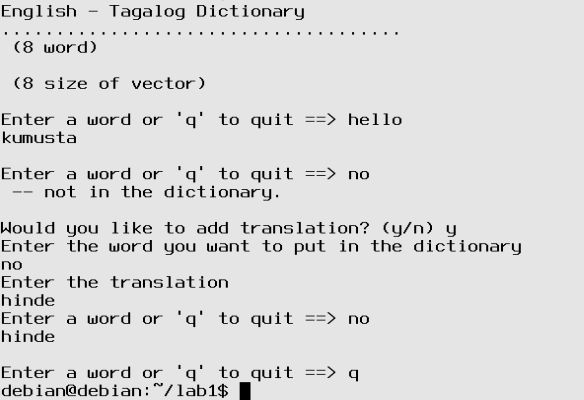
\includegraphics{../lab1.png}
 
\section{Class Index}
\subsection{Class List}
Here are the classes, structs, unions and interfaces with brief descriptions\+:\begin{DoxyCompactList}
\item\contentsline{section}{\hyperlink{structENTRY}{E\+N\+T\+R\+Y} }{\pageref{structENTRY}}{}
\end{DoxyCompactList}

\section{File Index}
\subsection{File List}
Here is a list of all files with brief descriptions\+:\begin{DoxyCompactList}
\item\contentsline{section}{\hyperlink{BuildListDirectly_8cpp}{Build\+List\+Directly.\+cpp} }{\pageref{BuildListDirectly_8cpp}}{}
\item\contentsline{section}{\hyperlink{destroyList_8cpp}{destroy\+List.\+cpp} }{\pageref{destroyList_8cpp}}{}
\item\contentsline{section}{\hyperlink{displayList_8cpp}{display\+List.\+cpp} }{\pageref{displayList_8cpp}}{}
\item\contentsline{section}{\hyperlink{Insert_8cpp}{Insert.\+cpp} }{\pageref{Insert_8cpp}}{}
\item\contentsline{section}{\hyperlink{InsertInOrder_8cpp}{Insert\+In\+Order.\+cpp} }{\pageref{InsertInOrder_8cpp}}{}
\item\contentsline{section}{\hyperlink{lab2_8h}{lab2.\+h} }{\pageref{lab2_8h}}{}
\item\contentsline{section}{\hyperlink{loadList_8cpp}{load\+List.\+cpp} }{\pageref{loadList_8cpp}}{}
\item\contentsline{section}{\hyperlink{loadList2_8cpp}{load\+List2.\+cpp} }{\pageref{loadList2_8cpp}}{}
\item\contentsline{section}{\hyperlink{loadList3_8cpp}{load\+List3.\+cpp} }{\pageref{loadList3_8cpp}}{}
\item\contentsline{section}{\hyperlink{main_8cpp}{main.\+cpp} }{\pageref{main_8cpp}}{}
\end{DoxyCompactList}

\section{Class Documentation}
\hypertarget{structENTRY}{\subsection{E\+N\+T\+R\+Y Struct Reference}
\label{structENTRY}\index{E\+N\+T\+R\+Y@{E\+N\+T\+R\+Y}}
}


{\ttfamily \#include $<$lab.\+h$>$}

\subsubsection*{Public Attributes}
\begin{DoxyCompactItemize}
\item 
string \hyperlink{structENTRY_a7dfcf0a0b27dc7cecf80565a615d6233}{word}
\item 
string \hyperlink{structENTRY_aeffa74a793268864bbbdf6a3645bf36a}{translation}
\end{DoxyCompactItemize}


\subsubsection{Member Data Documentation}
\hypertarget{structENTRY_aeffa74a793268864bbbdf6a3645bf36a}{\index{E\+N\+T\+R\+Y@{E\+N\+T\+R\+Y}!translation@{translation}}
\index{translation@{translation}!E\+N\+T\+R\+Y@{E\+N\+T\+R\+Y}}
\paragraph[{translation}]{\setlength{\rightskip}{0pt plus 5cm}string E\+N\+T\+R\+Y\+::translation}}\label{structENTRY_aeffa74a793268864bbbdf6a3645bf36a}
\hypertarget{structENTRY_a7dfcf0a0b27dc7cecf80565a615d6233}{\index{E\+N\+T\+R\+Y@{E\+N\+T\+R\+Y}!word@{word}}
\index{word@{word}!E\+N\+T\+R\+Y@{E\+N\+T\+R\+Y}}
\paragraph[{word}]{\setlength{\rightskip}{0pt plus 5cm}string E\+N\+T\+R\+Y\+::word}}\label{structENTRY_a7dfcf0a0b27dc7cecf80565a615d6233}


The documentation for this struct was generated from the following file\+:\begin{DoxyCompactItemize}
\item 
\hyperlink{lab_8h}{lab.\+h}\end{DoxyCompactItemize}

\section{File Documentation}
\hypertarget{foundWord_8cpp}{\subsection{found\+Word.\+cpp File Reference}
\label{foundWord_8cpp}\index{found\+Word.\+cpp@{found\+Word.\+cpp}}
}
{\ttfamily \#include \char`\"{}lab.\+h\char`\"{}}\\*
Include dependency graph for found\+Word.\+cpp\+:\nopagebreak
\begin{figure}[H]
\begin{center}
\leavevmode
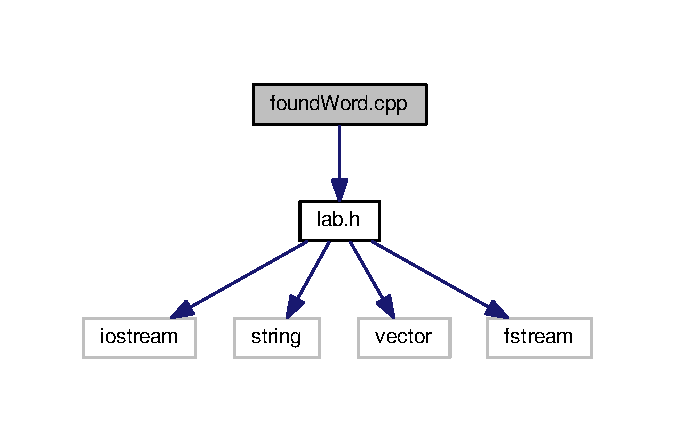
\includegraphics[width=324pt]{foundWord_8cpp__incl}
\end{center}
\end{figure}
\subsubsection*{Functions}
\begin{DoxyCompactItemize}
\item 
bool \hyperlink{foundWord_8cpp_abd296b13cd9c2eb14ca4bb5eae9766b3}{found\+Word} (const vector$<$ \hyperlink{structENTRY}{E\+N\+T\+R\+Y} $>$ \&dict, const string \&word, string \&translation)
\end{DoxyCompactItemize}


\subsubsection{Function Documentation}
\hypertarget{foundWord_8cpp_abd296b13cd9c2eb14ca4bb5eae9766b3}{\index{found\+Word.\+cpp@{found\+Word.\+cpp}!found\+Word@{found\+Word}}
\index{found\+Word@{found\+Word}!found\+Word.\+cpp@{found\+Word.\+cpp}}
\paragraph[{found\+Word}]{\setlength{\rightskip}{0pt plus 5cm}bool found\+Word (
\begin{DoxyParamCaption}
\item[{const vector$<$ {\bf E\+N\+T\+R\+Y} $>$ \&}]{dict, }
\item[{const string \&}]{word, }
\item[{string \&}]{translation}
\end{DoxyParamCaption}
)}}\label{foundWord_8cpp_abd296b13cd9c2eb14ca4bb5eae9766b3}

\begin{DoxyCode}
19 \{
20     \textcolor{keywordtype}{bool} found = \textcolor{keyword}{false}; \textcolor{comment}{//if the word is not found, it will return false}
21     \textcolor{comment}{//integer for the for loop and len is for the length of the vector}
22     \textcolor{keywordtype}{int} i, len = dict.size();
23     \textcolor{comment}{/*for loop which is needed to find the word in dictionary}
24 \textcolor{comment}{     which in turn gives the translation of the word*/}
25     \textcolor{keywordflow}{for} (i = 0; !found && i < len; i++) \{
26         \textcolor{keywordflow}{if} (dict[i].word == word)\{
27             translation = dict[i].translation;
28             found = \textcolor{keyword}{true};
29         \}\textcolor{comment}{//end of if}
30     \} \textcolor{comment}{//end of for}
31     \textcolor{keywordflow}{return} found; \textcolor{comment}{//returns the translation to user for it to be output}
32 \} \textcolor{comment}{//end of bool}
\end{DoxyCode}

\hypertarget{lab_8cpp}{\subsection{lab.\+cpp File Reference}
\label{lab_8cpp}\index{lab.\+cpp@{lab.\+cpp}}
}
{\ttfamily \#include \char`\"{}lab.\+h\char`\"{}}\\*
Include dependency graph for lab.\+cpp\+:\nopagebreak
\begin{figure}[H]
\begin{center}
\leavevmode
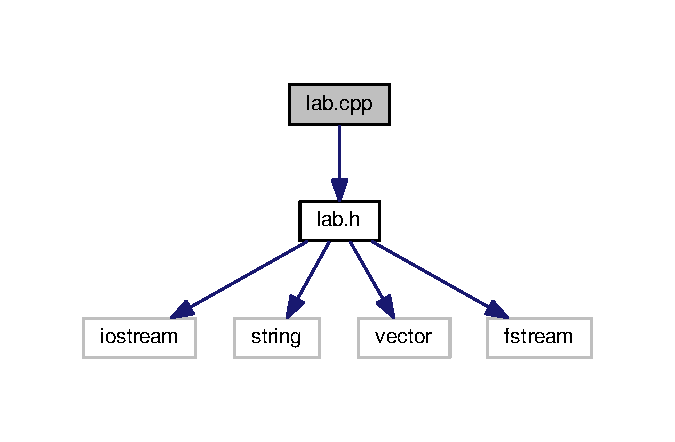
\includegraphics[width=324pt]{lab_8cpp__incl}
\end{center}
\end{figure}
\subsubsection*{Functions}
\begin{DoxyCompactItemize}
\item 
ostream \& \hyperlink{lab_8cpp_a2db0e63dc2d444c8135d1ef721a3297a}{operator$<$$<$} (ostream \&o, \hyperlink{structENTRY}{E\+N\+T\+R\+Y} \&e)
\item 
istream \& \hyperlink{lab_8cpp_ad328da1c67672d9165af2d1d7c7fa913}{operator$>$$>$} (istream \&i, \hyperlink{structENTRY}{E\+N\+T\+R\+Y} \&e)
\end{DoxyCompactItemize}


\subsubsection{Function Documentation}
\hypertarget{lab_8cpp_a2db0e63dc2d444c8135d1ef721a3297a}{\index{lab.\+cpp@{lab.\+cpp}!operator$<$$<$@{operator$<$$<$}}
\index{operator$<$$<$@{operator$<$$<$}!lab.\+cpp@{lab.\+cpp}}
\paragraph[{operator$<$$<$}]{\setlength{\rightskip}{0pt plus 5cm}ostream\& operator$<$$<$ (
\begin{DoxyParamCaption}
\item[{ostream \&}]{o, }
\item[{{\bf E\+N\+T\+R\+Y} \&}]{e}
\end{DoxyParamCaption}
)}}\label{lab_8cpp_a2db0e63dc2d444c8135d1ef721a3297a}

\begin{DoxyCode}
19 \{
20     o << e.\hyperlink{structENTRY_a7dfcf0a0b27dc7cecf80565a615d6233}{word} << \textcolor{stringliteral}{"\(\backslash\)t"};
21     o << e.\hyperlink{structENTRY_aeffa74a793268864bbbdf6a3645bf36a}{translation} << endl;
22     \textcolor{keywordflow}{return} o;
23 \}
\end{DoxyCode}
\hypertarget{lab_8cpp_ad328da1c67672d9165af2d1d7c7fa913}{\index{lab.\+cpp@{lab.\+cpp}!operator$>$$>$@{operator$>$$>$}}
\index{operator$>$$>$@{operator$>$$>$}!lab.\+cpp@{lab.\+cpp}}
\paragraph[{operator$>$$>$}]{\setlength{\rightskip}{0pt plus 5cm}istream\& operator$>$$>$ (
\begin{DoxyParamCaption}
\item[{istream \&}]{i, }
\item[{{\bf E\+N\+T\+R\+Y} \&}]{e}
\end{DoxyParamCaption}
)}}\label{lab_8cpp_ad328da1c67672d9165af2d1d7c7fa913}

\begin{DoxyCode}
26 \{
27     i >> e.\hyperlink{structENTRY_a7dfcf0a0b27dc7cecf80565a615d6233}{word} >> e.\hyperlink{structENTRY_aeffa74a793268864bbbdf6a3645bf36a}{translation};
28 \}
\end{DoxyCode}

\hypertarget{lab_8h}{\subsection{lab.\+h File Reference}
\label{lab_8h}\index{lab.\+h@{lab.\+h}}
}
{\ttfamily \#include \char`\"{}config.\+h\char`\"{}}\\*
{\ttfamily \#include $<$F\+L/\+Fl\+\_\+\+Cairo\+\_\+\+Window.\+H$>$}\\*
{\ttfamily \#include $<$F\+L/\+Fl\+\_\+\+Input.\+H$>$}\\*
{\ttfamily \#include $<$F\+L/\+Fl\+\_\+\+Button.\+H$>$}\\*
{\ttfamily \#include $<$F\+L/fl\+\_\+ask.\+H$>$}\\*
{\ttfamily \#include $<$iostream$>$}\\*
{\ttfamily \#include $<$F\+L/\+Fl\+\_\+\+Output.\+H$>$}\\*
{\ttfamily \#include $<$sstream$>$}\\*
{\ttfamily \#include $<$iomanip$>$}\\*
{\ttfamily \#include $<$F\+L/\+Fl\+\_\+\+Text\+\_\+\+Display.\+H$>$}\\*
{\ttfamily \#include $<$F\+L/\+Fl\+\_\+\+Text\+\_\+\+Buffer.\+H$>$}\\*
Include dependency graph for lab.\+h\+:\nopagebreak
\begin{figure}[H]
\begin{center}
\leavevmode
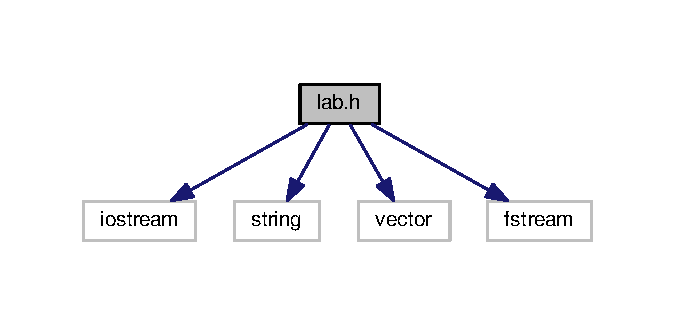
\includegraphics[width=350pt]{lab_8h__incl}
\end{center}
\end{figure}
This graph shows which files directly or indirectly include this file\+:\nopagebreak
\begin{figure}[H]
\begin{center}
\leavevmode
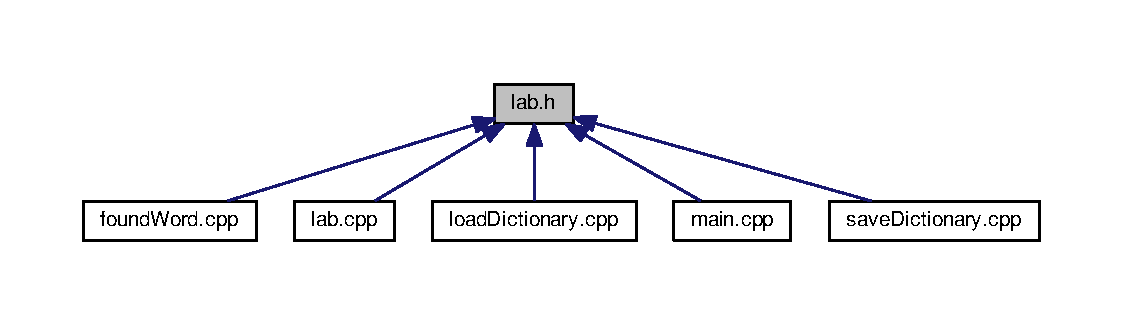
\includegraphics[width=350pt]{lab_8h__dep__incl}
\end{center}
\end{figure}
\subsubsection*{Functions}
\begin{DoxyCompactItemize}
\item 
void \hyperlink{lab_8h_a547f84331a8c529348e1130ca169c69c}{order\+\_\+cb} (void $\ast$, void $\ast$)
\item 
void \hyperlink{lab_8h_abb6fd11336b6e04e134b70abc225a8f6}{cook\+\_\+cb} (void $\ast$)
\item 
void \hyperlink{lab_8h_a13ed8751dfa95731ad8930762493b16b}{timer} (void $\ast$)
\end{DoxyCompactItemize}
\subsubsection*{Variables}
\begin{DoxyCompactItemize}
\item 
Fl\+\_\+\+Input $\ast$ \hyperlink{lab_8h_abf805c82a90897837d1c26ef915f1cd6}{pizza}
\item 
Fl\+\_\+\+Output $\ast$ \hyperlink{lab_8h_a05c7f6e86cca5f4d0ebf44d1f5042c37}{watch}
\item 
Fl\+\_\+\+Text\+\_\+\+Buffer $\ast$ \hyperlink{lab_8h_aea2b8efadc87a819fe57c311d668e504}{buff}
\item 
Fl\+\_\+\+Text\+\_\+\+Display $\ast$ \hyperlink{lab_8h_a23f917547a833922fd6bc8797cc04ee1}{order\+Q}
\end{DoxyCompactItemize}


\subsubsection{Function Documentation}
\hypertarget{lab_8h_abb6fd11336b6e04e134b70abc225a8f6}{\index{lab.\+h@{lab.\+h}!cook\+\_\+cb@{cook\+\_\+cb}}
\index{cook\+\_\+cb@{cook\+\_\+cb}!lab.\+h@{lab.\+h}}
\paragraph[{cook\+\_\+cb}]{\setlength{\rightskip}{0pt plus 5cm}void cook\+\_\+cb (
\begin{DoxyParamCaption}
\item[{void $\ast$}]{}
\end{DoxyParamCaption}
)}}\label{lab_8h_abb6fd11336b6e04e134b70abc225a8f6}

\begin{DoxyCode}
3 \{
4     \textcolor{comment}{//buff->text(pizza->value());}
5     
6     \textcolor{comment}{// temp solution, when it's cooked, put it}
7     \textcolor{comment}{// in the LLQueue; then here }
8     \textcolor{comment}{// use your new function that displays}
9     \textcolor{comment}{// what is in Q to create a string (with newlines)}
10     \textcolor{comment}{// in it, return it here and siplay that in the buffer}
11     
12 \}
\end{DoxyCode}
\hypertarget{lab_8h_a547f84331a8c529348e1130ca169c69c}{\index{lab.\+h@{lab.\+h}!order\+\_\+cb@{order\+\_\+cb}}
\index{order\+\_\+cb@{order\+\_\+cb}!lab.\+h@{lab.\+h}}
\paragraph[{order\+\_\+cb}]{\setlength{\rightskip}{0pt plus 5cm}void order\+\_\+cb (
\begin{DoxyParamCaption}
\item[{void $\ast$}]{, }
\item[{void $\ast$}]{}
\end{DoxyParamCaption}
)}}\label{lab_8h_a547f84331a8c529348e1130ca169c69c}

\begin{DoxyCode}
3 \{
4     fl\_alert(\hyperlink{lab_8h_abf805c82a90897837d1c26ef915f1cd6}{pizza}->value());
5     \textcolor{comment}{// cook it}
6     Fl::add\_timeout(5,\hyperlink{cook__cb_8cpp_abb6fd11336b6e04e134b70abc225a8f6}{cook\_cb});
7 \}
\end{DoxyCode}
\hypertarget{lab_8h_a13ed8751dfa95731ad8930762493b16b}{\index{lab.\+h@{lab.\+h}!timer@{timer}}
\index{timer@{timer}!lab.\+h@{lab.\+h}}
\paragraph[{timer}]{\setlength{\rightskip}{0pt plus 5cm}void timer (
\begin{DoxyParamCaption}
\item[{void $\ast$}]{}
\end{DoxyParamCaption}
)}}\label{lab_8h_a13ed8751dfa95731ad8930762493b16b}

\begin{DoxyCode}
3 \{
4     \textcolor{comment}{//std::cout << "1 sec" << std::endl;}
5     \textcolor{keyword}{static} \textcolor{keywordtype}{int} s= 0; \textcolor{keyword}{static} \textcolor{keywordtype}{int} m = 0;
6     std::ostringstream oss; \textcolor{comment}{// don't discard the memory. }
7                                               \textcolor{comment}{// keep it so we can update t to the window}
8     s++;    \textcolor{keywordflow}{if}(s == 59) \{s = 0; m++; \}
9     oss << std::setfill(\textcolor{charliteral}{'0'});
10     oss << std::setw(2) << m << \textcolor{stringliteral}{":"} << std::setw(2) << s;
11     \textcolor{comment}{//oss << s;}
12     \hyperlink{lab_8h_a05c7f6e86cca5f4d0ebf44d1f5042c37}{watch}->value(oss.str().c\_str());
13     
14     \textcolor{comment}{// Here we could check if the Q's have pizza and drivers}
15     \textcolor{comment}{// ready for delivery every 10 seconds so we can see order}
16     \textcolor{comment}{// in Q     if (s % 10 == 0)}
17     \textcolor{keyword}{static} std::string str;
18     std::string pizzas[] = \{\textcolor{stringliteral}{"veggie"},\textcolor{stringliteral}{"pepperoni"},\textcolor{stringliteral}{"sausage"},\textcolor{stringliteral}{"hawaiian"}\};
19     \textcolor{keywordflow}{if}(s % 10 == 0)
20     \{
21         str += pizzas[s%4] += \textcolor{stringliteral}{"\(\backslash\)n"};
22         \hyperlink{lab_8h_aea2b8efadc87a819fe57c311d668e504}{buff}->text(str.c\_str());
23     \}
24     
25     Fl::repeat\_timeout(1,\hyperlink{timer_8cpp_a13ed8751dfa95731ad8930762493b16b}{timer});
26 \}
\end{DoxyCode}


\subsubsection{Variable Documentation}
\hypertarget{lab_8h_aea2b8efadc87a819fe57c311d668e504}{\index{lab.\+h@{lab.\+h}!buff@{buff}}
\index{buff@{buff}!lab.\+h@{lab.\+h}}
\paragraph[{buff}]{\setlength{\rightskip}{0pt plus 5cm}Fl\+\_\+\+Text\+\_\+\+Buffer$\ast$ buff}}\label{lab_8h_aea2b8efadc87a819fe57c311d668e504}
\hypertarget{lab_8h_a23f917547a833922fd6bc8797cc04ee1}{\index{lab.\+h@{lab.\+h}!order\+Q@{order\+Q}}
\index{order\+Q@{order\+Q}!lab.\+h@{lab.\+h}}
\paragraph[{order\+Q}]{\setlength{\rightskip}{0pt plus 5cm}Fl\+\_\+\+Text\+\_\+\+Display$\ast$ order\+Q}}\label{lab_8h_a23f917547a833922fd6bc8797cc04ee1}
\hypertarget{lab_8h_abf805c82a90897837d1c26ef915f1cd6}{\index{lab.\+h@{lab.\+h}!pizza@{pizza}}
\index{pizza@{pizza}!lab.\+h@{lab.\+h}}
\paragraph[{pizza}]{\setlength{\rightskip}{0pt plus 5cm}Fl\+\_\+\+Input$\ast$ pizza}}\label{lab_8h_abf805c82a90897837d1c26ef915f1cd6}
\hypertarget{lab_8h_a05c7f6e86cca5f4d0ebf44d1f5042c37}{\index{lab.\+h@{lab.\+h}!watch@{watch}}
\index{watch@{watch}!lab.\+h@{lab.\+h}}
\paragraph[{watch}]{\setlength{\rightskip}{0pt plus 5cm}Fl\+\_\+\+Output$\ast$ watch}}\label{lab_8h_a05c7f6e86cca5f4d0ebf44d1f5042c37}

\hypertarget{loadDictionary_8cpp}{\subsection{load\+Dictionary.\+cpp File Reference}
\label{loadDictionary_8cpp}\index{load\+Dictionary.\+cpp@{load\+Dictionary.\+cpp}}
}
{\ttfamily \#include \char`\"{}lab.\+h\char`\"{}}\\*
Include dependency graph for load\+Dictionary.\+cpp\+:\nopagebreak
\begin{figure}[H]
\begin{center}
\leavevmode
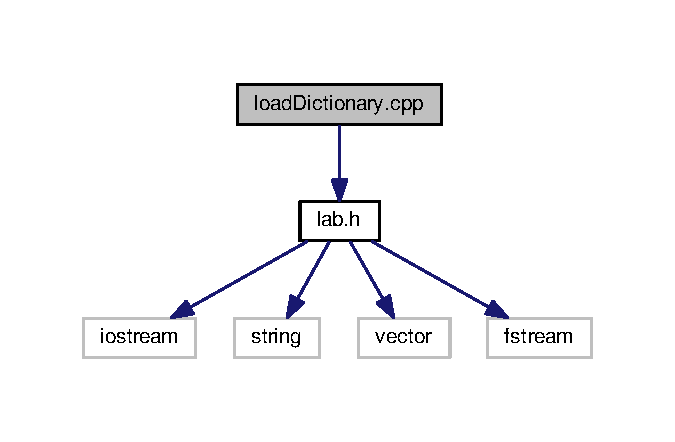
\includegraphics[width=324pt]{loadDictionary_8cpp__incl}
\end{center}
\end{figure}
\subsubsection*{Functions}
\begin{DoxyCompactItemize}
\item 
bool \hyperlink{loadDictionary_8cpp_a14d9a1d2cb42104c2d9cf01571b162a7}{load\+Dictionary} (string file\+Name, vector$<$ \hyperlink{structENTRY}{E\+N\+T\+R\+Y} $>$ \&dict)
\end{DoxyCompactItemize}


\subsubsection{Function Documentation}
\hypertarget{loadDictionary_8cpp_a14d9a1d2cb42104c2d9cf01571b162a7}{\index{load\+Dictionary.\+cpp@{load\+Dictionary.\+cpp}!load\+Dictionary@{load\+Dictionary}}
\index{load\+Dictionary@{load\+Dictionary}!load\+Dictionary.\+cpp@{load\+Dictionary.\+cpp}}
\paragraph[{load\+Dictionary}]{\setlength{\rightskip}{0pt plus 5cm}bool load\+Dictionary (
\begin{DoxyParamCaption}
\item[{string}]{file\+Name, }
\item[{vector$<$ {\bf E\+N\+T\+R\+Y} $>$ \&}]{dict}
\end{DoxyParamCaption}
)}}\label{loadDictionary_8cpp_a14d9a1d2cb42104c2d9cf01571b162a7}

\begin{DoxyCode}
20 \{   \textcolor{comment}{//integer needed for counting how many words are in dictionary}
21     \textcolor{keywordtype}{int} cnt = 0; 
22     \hyperlink{structENTRY}{ENTRY} e; \textcolor{comment}{//to access the vector ENTRY which contain word and translation}
23     ifstream inpFile(fileName.c\_str());
24     \textcolor{keywordflow}{if} (!inpFile) \textcolor{keywordflow}{return} \textcolor{keyword}{false}; \textcolor{comment}{//if file does not open, it will return false}
25     \textcolor{keywordtype}{string} title; \textcolor{comment}{//string to contain title}
26     getline(inpFile, title); \textcolor{comment}{//to get the title from the text file}
27     cout << title << endl; \textcolor{comment}{//to print the title of the program}
28     cout << \textcolor{stringliteral}{"....................................."} << endl;
29     \textcolor{keywordflow}{while} (inpFile >> e.\hyperlink{structENTRY_a7dfcf0a0b27dc7cecf80565a615d6233}{word} >> e.\hyperlink{structENTRY_aeffa74a793268864bbbdf6a3645bf36a}{translation}) \{
30         dict.push\_back(e);
31         inpFile.ignore(80, \textcolor{charliteral}{'\(\backslash\)n'}); \textcolor{comment}{//skip the rest of the line}
32         cnt++;
33     \}\textcolor{comment}{//end of while for inpFile}
34     
35     cout << \textcolor{stringliteral}{" ("} << cnt << \textcolor{stringliteral}{" words)\(\backslash\)n\(\backslash\)n"}; \textcolor{comment}{//prints out the number of words}
36     \textcolor{comment}{//prints out the number of vectors used}
37     cout << \textcolor{stringliteral}{" ("} << dict.size() << \textcolor{stringliteral}{" size of vector)\(\backslash\)n\(\backslash\)n"};
38     
39     \textcolor{keywordflow}{return} \textcolor{keyword}{true};
40 \} \textcolor{comment}{//end of bool loadDictionary}
\end{DoxyCode}

\hypertarget{main_8cpp}{\subsection{main.\+cpp File Reference}
\label{main_8cpp}\index{main.\+cpp@{main.\+cpp}}
}
{\ttfamily \#include \char`\"{}lab.\+h\char`\"{}}\\*
Include dependency graph for main.\+cpp\+:\nopagebreak
\begin{figure}[H]
\begin{center}
\leavevmode
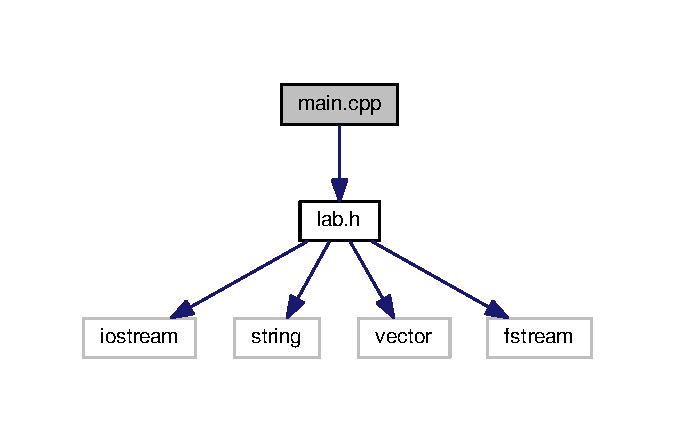
\includegraphics[width=350pt]{main_8cpp__incl}
\end{center}
\end{figure}
\subsubsection*{Functions}
\begin{DoxyCompactItemize}
\item 
int \hyperlink{main_8cpp_ae66f6b31b5ad750f1fe042a706a4e3d4}{main} ()
\end{DoxyCompactItemize}
\subsubsection*{Variables}
\begin{DoxyCompactItemize}
\item 
Fl\+\_\+\+Input $\ast$ \hyperlink{main_8cpp_abf805c82a90897837d1c26ef915f1cd6}{pizza}
\item 
Fl\+\_\+\+Output $\ast$ \hyperlink{main_8cpp_a05c7f6e86cca5f4d0ebf44d1f5042c37}{watch}
\item 
Fl\+\_\+\+Text\+\_\+\+Buffer $\ast$ \hyperlink{main_8cpp_aea2b8efadc87a819fe57c311d668e504}{buff}
\item 
Fl\+\_\+\+Text\+\_\+\+Display $\ast$ \hyperlink{main_8cpp_a23f917547a833922fd6bc8797cc04ee1}{order\+Q}
\end{DoxyCompactItemize}


\subsubsection{Function Documentation}
\hypertarget{main_8cpp_ae66f6b31b5ad750f1fe042a706a4e3d4}{\index{main.\+cpp@{main.\+cpp}!main@{main}}
\index{main@{main}!main.\+cpp@{main.\+cpp}}
\paragraph[{main}]{\setlength{\rightskip}{0pt plus 5cm}int main (
\begin{DoxyParamCaption}
{}
\end{DoxyParamCaption}
)}}\label{main_8cpp_ae66f6b31b5ad750f1fe042a706a4e3d4}

\begin{DoxyCode}
10 \{
11     Fl\_Cairo\_Window cw(400,300); \textcolor{comment}{// width & height of window}
12     cw.label(\textcolor{stringliteral}{"Pizza Deliveries Extravaganja"}); \textcolor{comment}{// title of your cairo window}
13     \textcolor{comment}{//cw.color(FL\_GREEN);}
14     
15     \hyperlink{main_8cpp_abf805c82a90897837d1c26ef915f1cd6}{pizza} = \textcolor{keyword}{new} Fl\_Input(190, 20, 100, 20, \textcolor{stringliteral}{"pizza:"});
16     \hyperlink{main_8cpp_abf805c82a90897837d1c26ef915f1cd6}{pizza}->labelcolor(FL\_BLUE);
17     
18     \hyperlink{main_8cpp_aea2b8efadc87a819fe57c311d668e504}{buff} = \textcolor{keyword}{new} Fl\_Text\_Buffer();
19     \hyperlink{main_8cpp_a23f917547a833922fd6bc8797cc04ee1}{orderQ} = \textcolor{keyword}{new} Fl\_Text\_Display(100,100,100,100,\textcolor{stringliteral}{"Order Q"});
20     \hyperlink{main_8cpp_a23f917547a833922fd6bc8797cc04ee1}{orderQ}->buffer(\hyperlink{main_8cpp_aea2b8efadc87a819fe57c311d668e504}{buff});
21     
22     \hyperlink{main_8cpp_a05c7f6e86cca5f4d0ebf44d1f5042c37}{watch} = \textcolor{keyword}{new} Fl\_Output(70,20,50,20,\textcolor{stringliteral}{"seconds:"});
23     
24     Fl\_Button b(330, 60, 50, 20, \textcolor{stringliteral}{"Order:"});
25     b.callback((Fl\_Callback*)\hyperlink{lab_8h_a547f84331a8c529348e1130ca169c69c}{order\_cb});
26     
27     cw.show();
28     Fl::add\_timeout(1,\hyperlink{lab_8h_a13ed8751dfa95731ad8930762493b16b}{timer});
29     \textcolor{keywordflow}{return} Fl::run();
30 \}
\end{DoxyCode}


\subsubsection{Variable Documentation}
\hypertarget{main_8cpp_aea2b8efadc87a819fe57c311d668e504}{\index{main.\+cpp@{main.\+cpp}!buff@{buff}}
\index{buff@{buff}!main.\+cpp@{main.\+cpp}}
\paragraph[{buff}]{\setlength{\rightskip}{0pt plus 5cm}Fl\+\_\+\+Text\+\_\+\+Buffer$\ast$ buff}}\label{main_8cpp_aea2b8efadc87a819fe57c311d668e504}
\hypertarget{main_8cpp_a23f917547a833922fd6bc8797cc04ee1}{\index{main.\+cpp@{main.\+cpp}!order\+Q@{order\+Q}}
\index{order\+Q@{order\+Q}!main.\+cpp@{main.\+cpp}}
\paragraph[{order\+Q}]{\setlength{\rightskip}{0pt plus 5cm}Fl\+\_\+\+Text\+\_\+\+Display$\ast$ order\+Q}}\label{main_8cpp_a23f917547a833922fd6bc8797cc04ee1}
\hypertarget{main_8cpp_abf805c82a90897837d1c26ef915f1cd6}{\index{main.\+cpp@{main.\+cpp}!pizza@{pizza}}
\index{pizza@{pizza}!main.\+cpp@{main.\+cpp}}
\paragraph[{pizza}]{\setlength{\rightskip}{0pt plus 5cm}Fl\+\_\+\+Input$\ast$ pizza}}\label{main_8cpp_abf805c82a90897837d1c26ef915f1cd6}
\hypertarget{main_8cpp_a05c7f6e86cca5f4d0ebf44d1f5042c37}{\index{main.\+cpp@{main.\+cpp}!watch@{watch}}
\index{watch@{watch}!main.\+cpp@{main.\+cpp}}
\paragraph[{watch}]{\setlength{\rightskip}{0pt plus 5cm}Fl\+\_\+\+Output$\ast$ watch}}\label{main_8cpp_a05c7f6e86cca5f4d0ebf44d1f5042c37}

\hypertarget{saveDictionary_8cpp}{\subsection{save\+Dictionary.\+cpp File Reference}
\label{saveDictionary_8cpp}\index{save\+Dictionary.\+cpp@{save\+Dictionary.\+cpp}}
}
{\ttfamily \#include \char`\"{}lab.\+h\char`\"{}}\\*
Include dependency graph for save\+Dictionary.\+cpp\+:\nopagebreak
\begin{figure}[H]
\begin{center}
\leavevmode
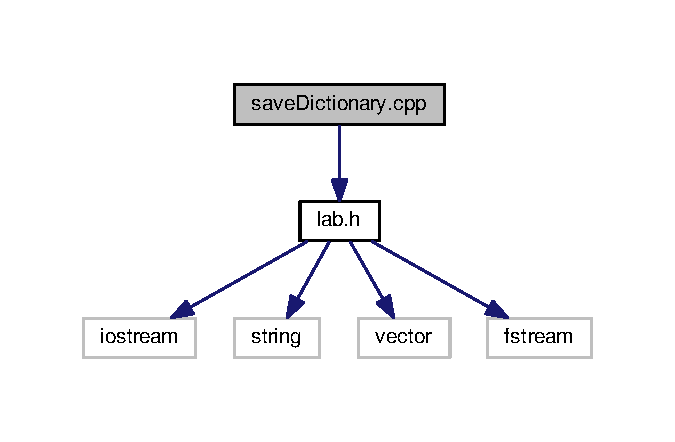
\includegraphics[width=324pt]{saveDictionary_8cpp__incl}
\end{center}
\end{figure}
\subsubsection*{Functions}
\begin{DoxyCompactItemize}
\item 
bool \hyperlink{saveDictionary_8cpp_abec3741182deca1e3f68c16664818602}{save\+Dictionary} (string file\+Name, vector$<$ \hyperlink{structENTRY}{E\+N\+T\+R\+Y} $>$ \&dict)
\end{DoxyCompactItemize}


\subsubsection{Function Documentation}
\hypertarget{saveDictionary_8cpp_abec3741182deca1e3f68c16664818602}{\index{save\+Dictionary.\+cpp@{save\+Dictionary.\+cpp}!save\+Dictionary@{save\+Dictionary}}
\index{save\+Dictionary@{save\+Dictionary}!save\+Dictionary.\+cpp@{save\+Dictionary.\+cpp}}
\paragraph[{save\+Dictionary}]{\setlength{\rightskip}{0pt plus 5cm}bool save\+Dictionary (
\begin{DoxyParamCaption}
\item[{string}]{file\+Name, }
\item[{vector$<$ {\bf E\+N\+T\+R\+Y} $>$ \&}]{dict}
\end{DoxyParamCaption}
)}}\label{saveDictionary_8cpp_abec3741182deca1e3f68c16664818602}

\begin{DoxyCode}
20 \{   
21     \textcolor{keywordtype}{string} input; \textcolor{comment}{//to get user's input}
22     \hyperlink{structENTRY}{ENTRY} e; \textcolor{comment}{//to access the vector ENTRY}
23     fstream saveFile; \textcolor{comment}{//object to access text file 'dict.dat'}
24     saveFile.open(fileName.c\_str(), ios::app); \textcolor{comment}{//to open text file}
25     \textcolor{comment}{//to tell the user the word is not in the dictionary}
26     cout << e.\hyperlink{structENTRY_a7dfcf0a0b27dc7cecf80565a615d6233}{word} << \textcolor{stringliteral}{" -- not in the dictionary.\(\backslash\)n\(\backslash\)n"};
27     cout << \textcolor{stringliteral}{"Would you like to add translation? (y/n) "};
28     cin >> input; \textcolor{comment}{//taking in user's input}
29     \textcolor{comment}{/*if loop that if the user wants to add their word and translation}
30 \textcolor{comment}{      into the dictionary, they must type 'y', if not, anything else}
31 \textcolor{comment}{      to continue the code.}
32 \textcolor{comment}{    */}
33             \textcolor{keywordflow}{if}(input == \textcolor{stringliteral}{"y"})
34                 \{   
35                     \hyperlink{structENTRY}{ENTRY} e;
36                     cout << \textcolor{stringliteral}{"Enter the word you want to put in the dictionary "} << endl;
37                     cin >> e.\hyperlink{structENTRY_a7dfcf0a0b27dc7cecf80565a615d6233}{word}; \textcolor{comment}{//take in user input for word}
38                     cout << \textcolor{stringliteral}{"Enter the translation: "} << endl;
39                     cin >> e.\hyperlink{structENTRY_aeffa74a793268864bbbdf6a3645bf36a}{translation}; \textcolor{comment}{//take in user input for translation}
40                     dict.push\_back(e); \textcolor{comment}{// enters user input to last element of vector}
41                     \textcolor{comment}{//saves user's input into the text file}
42                     saveFile << e.\hyperlink{structENTRY_a7dfcf0a0b27dc7cecf80565a615d6233}{word} << \textcolor{stringliteral}{" "} << e.\hyperlink{structENTRY_aeffa74a793268864bbbdf6a3645bf36a}{translation} << endl;
43 
44                 \}
45 \}
\end{DoxyCode}

\hypertarget{specification_8dox}{\subsection{specification.\+dox File Reference}
\label{specification_8dox}\index{specification.\+dox@{specification.\+dox}}
}

%--- End generated contents ---

% Index
\newpage
\phantomsection
\addcontentsline{toc}{section}{Index}
\printindex

\end{document}
